\chapter{Feature Engineering}

\section{The Acoustic Manifold}
The core of our tabular modeling approach is the extraction of a 100-dimensional feature vector from the raw audio signal. This "Acoustic Manifold" captures the mathematical representation of the sound across time, frequency, and harmonic domains. The 100 features are derived from 25 base acoustic metrics, each expanded by four statistical moments: mean, standard deviation, maximum, and minimum.

\section{Feature Categories}

\subsection{Mel-Frequency Cepstral Coefficients (MFCCs)}
MFCCs are the standard in audio processing, representing the short-term power spectrum of a sound. We extracted 13 MFCC coefficients, providing a detailed view of the spectral envelope. For each coefficient, we computed:
\begin{itemize}
    \item \textbf{Statistical Expansion:} Mean, standard deviation, maximum, and minimum values across the time-axis, resulting in 52 MFCC-based features.
\end{itemize}

\subsection{Spectral Shape Features}
Beyond MFCCs, we extracted several critical spectral metrics, each expanded with the same four statistical moments (12 features total):
\begin{itemize}
    \item \textbf{Spectral Centroid:} Indicates where the "center of mass" of the spectrum is located (related to brightness).
    \item \textbf{Spectral Bandwidth:} Describes the range of frequencies the signal covers.
    \item \textbf{Spectral Rolloff:} The frequency below which 85\% of the spectral power is concentrated.
\end{itemize}

\subsection{Spectral Contrast}
Spectral Contrast measures the difference in power between peaks and valleys across 7 frequency bands. This feature is expanded into 28 statistical columns and has proven highly effective for mechanical anomaly detection by capturing harmonic shifts.

\subsection{Temporal Features}
The time-domain characteristics are captured by 8 features (2 metrics $\times$ 4 stats):
\begin{itemize}
    \item \textbf{Zero-Crossing Rate (ZCR):} Captures the frequency at which the signal changes sign. High ZCR is often associated with high-frequency mechanical noise.
    \item \textbf{RMS Energy:} Measures the overall power/loudness of the recording.
\end{itemize}
All temporal features are likewise expanded into mean, std, max, and min statistics to capture both global properties and transient peaks.

\section{Feature Importance and Pruning}
To optimize for edge-deployment (where memory and CPU cycles are limited), we conducted a feature importance study using a Random Forest model with 50 estimators. 

\begin{figure}[H]
    \centering
    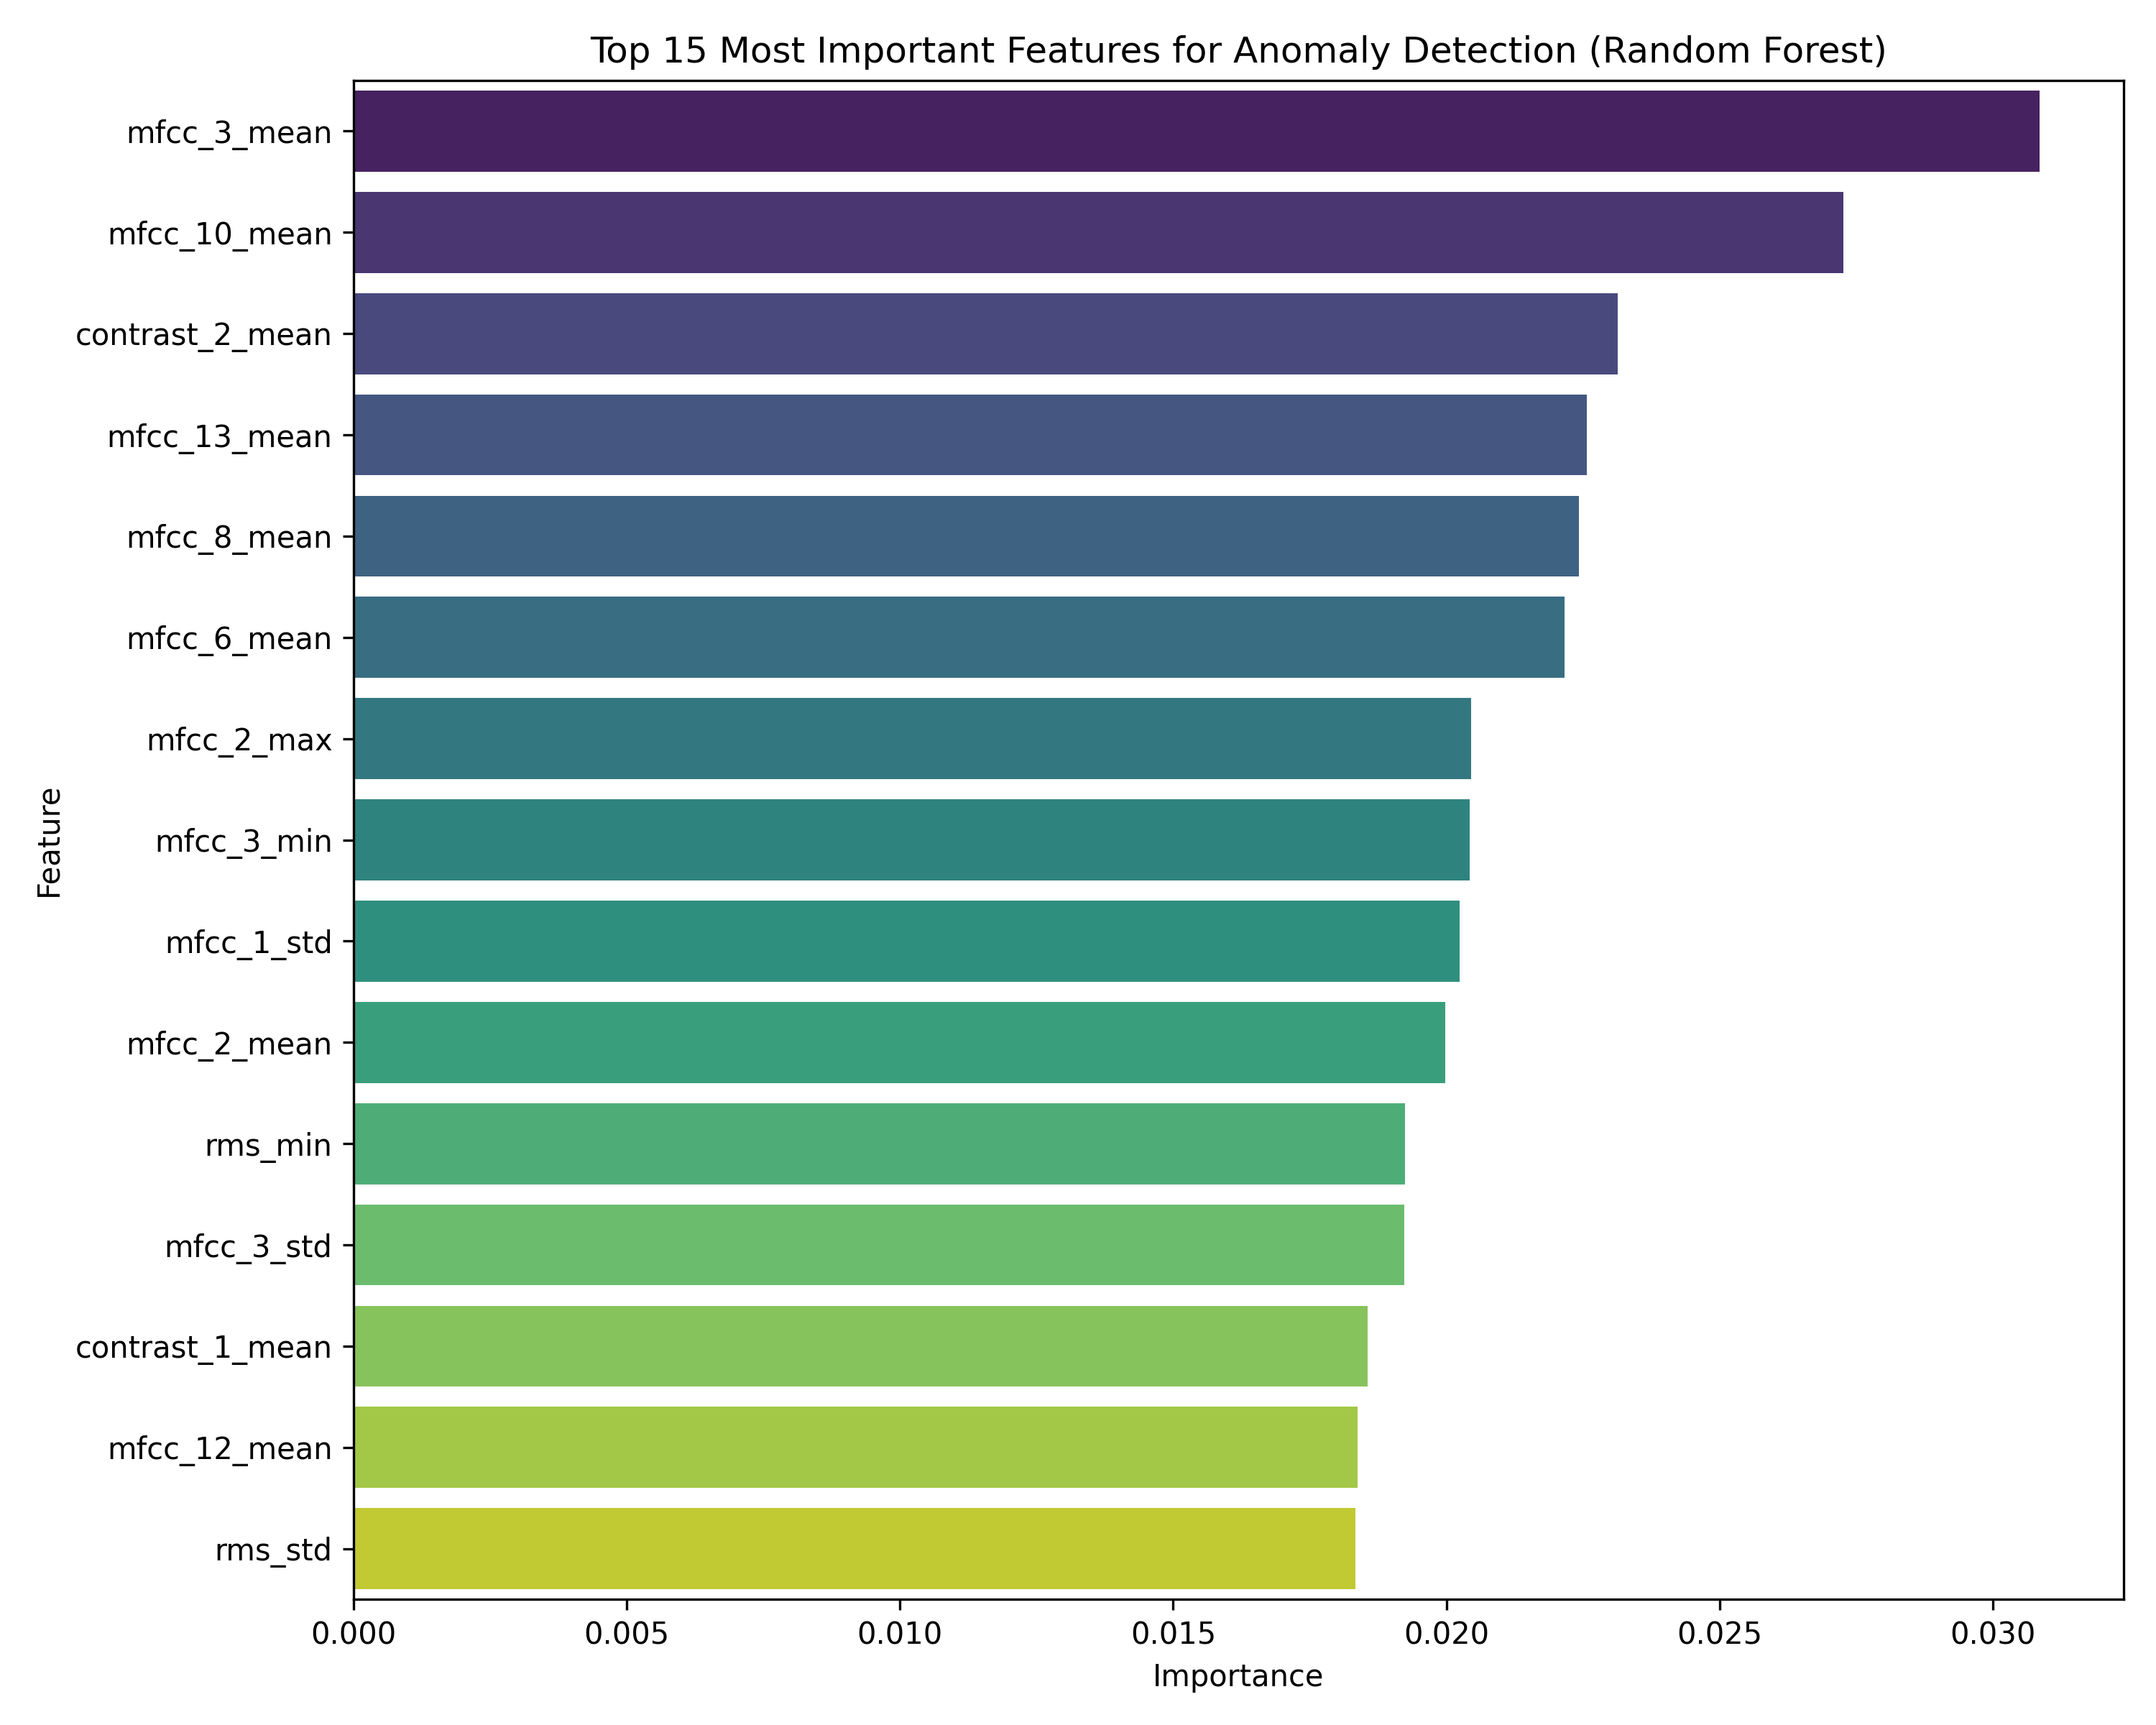
\includegraphics[width=0.8\textwidth]{figures/feature_importance.png}
    \caption{Top 20 Most Predictive Acoustic Features}
    \label{fig:feat_imp}
\end{figure}

By retaining only the Top 40 features, we were able to reduce the model size significantly while maintaining a high F1-score. This pruning process is essential for deploying the model on low-power industrial gateways.

\section{Normalization and Scaling}
Before training, all features are passed through a \texttt{StandardScaler} to ensure they have zero mean and unit variance. This step is critical for algorithms like SVM and Deep Learning, though less impactful for the gradient-boosted trees used in our final XGBoost model.
